\subsection{Clustering}\label{sec:clustering}
%Another way of optimising the computation of the link model is to introduce clustering of nodes, used to reduce the amount of links required for the link model computation. 
The second option for optimising the computation of the link model, is to introduce clustering of nodes. As mentioned in \autoref{sec:pathloss}, links existing in the same physical environment should experience similar shadow fading \gls{pathloss}. This means that we are be able to cluster nodes with a minimum loss of precision, provided that we minimise difference of the correlation (the angle) between links, before and after clustering.

%minimise the difference of the angles between links before and after clustering (correlation)

%This means that we should be able to compute clusters of nodes, and use the clusters to faster compute the link model of multiple nodes at the same time, as we would, depending on the number of clusters, have a far smaller link matrix. \medbreak

%For our purposes, we have chosen to use a density-based clustering algorithm, more specifically the \gls{optics} algorithm (\autoref{algo:optics}). The idea behind density-based clustering is that for every node in a cluster, the neighbourhood, within a given radius, has to contain at least a minimum number of other nodes~\cite[p.~50]{Ankerst:1999:OOP:304182.304187}. A set of nodes in a network, $\textbf{N} \subseteq \mathcal{X}$, along with a distance parameter $\varepsilon$, denoting the maximum radius of a nodes neighbourhood, and $MinNodes \geq 2$ denoting the minimum number of nodes required to form a cluster, such that a single node will not be considered a cluster. The goal is to find a set of clusters, $C$, such that we are able to form a new network with the centroids of our set of clusters, as well any outlying node not contained in a cluster, $\text{NOISE} \subseteq \textbf{N}$, while minimising the radius of the clusters.

%\subsubsection{Metric Space}
% Minimise the diameter using parameters
% Maximum diameter as input, give me the smallest number of k-nodes, such that every other node is within the diameter of at least one node.
% Output: Some number of nodes, which is the smallest possible diameter

%metric space
\subsection{Metric Space}
A metric space is a pair $( \mathcal{X}, d )$ where $ \mathcal{X} $ is a set and $\textbf{d}:\mathcal{X} \times \mathcal{X} \rightarrow [0, \infty )$ is a metric, satisfying the following axioms:

\begin{itemize}
    \item Reflexivity: $d(x, y) = 0 \Longleftrightarrow x = y$
    \item Symmetry: $d(x, y) = d(y, x)$
    \item Triangle inequality: $d(x, z) \leq d(x, y) + d(y, z)$
\end{itemize}

Our chosen metric space is $\mathbb{R}^2$ using Euclidean distance.

%$\mathbb{R}^2$

\subsubsection{Problem Statement}

%A set $\textbf{N} \subseteq \mathcal{X}$, is provided together with parameters $\varepsilon$. The goal is to find a subset of clusters, such that the maximum angle between any node to nodes in the cluster is minimised. 
A set $\textbf{N} \subseteq \mathcal{X}$, is provided together with a parameter $k$, $k \leq |\textbf{N}|$. Initially, the set $\textbf{N}$ is a set of clusters, each containing a single node. The goal is to find a set of clusters, such that we can reduce the computational time required for computing the link model, while minimising the loss of precision in the stochastic shadow fading part. We minimise the loss of precision by minimising the difference of the correlation ($\Delta\theta$) between links to any node in a cluster, to the centroid of the cluster. The problem is defined as follows: \smallbreak

%This correlation difference is computed using the autocorrelation function from \autoref{eq:pathlossautocorrelation}.


% \autoref{figure:clusteringgoal} contains an example of this
%For example, we want to minimise the difference $\Delta\theta$ between the links $l_{n,u}$, $l_{n, c}$, in relation to the link $l_{n,m}$ in \autoref{figure:clusteringgoal}. The difference is computed using the autocorrelation function from \autoref{eq:pathlossautocorrelation}: $\Delta\theta = r(l_{n,m}, l_{n,u}) - r(l_{n,m},l_{n,c})$, where $u \in c$, $n \not\in c$, $m \not\in c$.

%The goal is to find a 
%subset of clusters, such that the difference of the correlation between ($\Delta\theta$) links to any node in a cluster, to the centroid of the cluster, is minimised, while reducing the number of clusters, thus reducing the computational time required to compute the link model, while minimising the loss of precision.

%s an example, in \autoref{figure:clusteringgoal}, we want to minimise the difference $\Delta\theta$, between the links $l_{n,u}$, $l_{n, C}$, in relation to the link $l_{n,m}$, or $\Delta\theta = r(l_{n,m}, l_{n,u}) - r(l_{n,m},l_{n,C})$, where $u \in C$, $n \not\in C$, $m \not\in C$, and $r$ is the autocorrelation function from \autoref{eq:pathlossautocorrelation}. 

%such that the difference between an angle any node from outside the cluster to the centroid of the cluster, and the original node in the cluster is minimised.
%\autoref{figure:clusteringgoal} demonstrate an example of this, where we see three clusters of nodes.
%$\delta\theta$

%such that the difference in correlation between links is minimised, while maximising the number of clusters. 

%Minimise the difference between the original correlation matrix, and the new correlation matrix created using the centroid of the clusters.


For a metric space $(\mathcal{X}, d)$,
\begin{itemize}
    \item Input: A set $\textbf{N} \subseteq \mathcal{X}$ and a parameter $k$, $k \leq |\textbf{N}|$.
    \item Output: A set of clusters $C \subseteq 2^{\textbf{N}}$, such that
    \begin{enumerate}
        \item $\bigcup\limits_{x \ \in \ C}x = \textbf{N}$,
        \item $\forall x, y \in C, \ \text{if} \ x \neq y \ \text{then} \ x \cap y = \emptyset$, and
        \item $|C| \leq k$
    \end{enumerate} 
    \item Goal: Minimise the $\Delta\theta(C)$ function:\smallbreak $\Delta\theta(C) = \mathlarger{\sum}\limits_{n_1, n_2, n_3 \ \in \ \textbf{N}} \left( r(l_{n_1,n_2}, l_{n_1,n_3}) - r(l_{C(n_1),C(n_2)}, l_{C(n_1),C(n_3)}) \right)^2$ 

    % \item Input: a set $\textbf{N} \subseteq \mathcal{X}$, and a parameter $\varepsilon$.
    %       %    \item Output: a set of clusters $C$ where, for each nodes in the cluster, the neighbourhood of a given radius $\varepsilon$ of the nodes has to contain at least a minimum number of nodes $MinNodes$.
    % \item Output: a set of clusters $C$. % færre elementer end det set vi startede med
    % \item Goal: minimise the difference in correlation, $\Delta\theta$, between links $l_{n,c}$, $l_{n,u}$, with relation to $l_{n, m}$, for any $c \in C$, $u \in c$, $n \not\in c$, and $m \not\in c$, where $n \neq m$.

          %$\forall c \in C, \forall u \in c, \forall m \not\in c, \forall n \not\in c, $

          %$\Delta\theta$, $\forall c \in C,  $  $\Delta\theta = r(l_{n,m}, l_{n,u}) - r(l_{n,m},l_{n,C})$
          %    \item Goal: minimise the cost $r^C_\infty(\textbf{N}) = \max\limits_{n \in \textbf{N}} d(n, C)$.
          %\item Goal: minimise the size of the network by creating a new network consisting of the set of nodes $centroids(C) \cup \text{NOISE}$
          %\item Goal: Minimise the cost $r^C_\infty(\textbf{P}) = \max{p \in \textbf{P}} d(p, C)$
\end{itemize}

%\todo[inline]{How to describe the goal? Is it the goal of the particular clustering algorithm, or our goal for using the clustering algorithm? In the second case, the goal is to reduce the number of overall nodes in the network, by creating clusters of nodes very close to each other, and using the centroid of the clusters for the link model.}

\begin{figure}[ht]
    \centering
    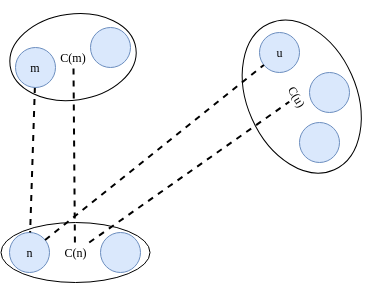
\includegraphics[width=.5\textwidth]{figures/clustering/clustering.png}
    \caption{Minimising the difference of the correlation ($\Delta\theta$) between links to nodes in a cluster to the centroid of the cluster.}
    \label{figure:clusteringgoal}
\end{figure}

\subsubsection{Approximation using OPTICS}
We have chosen a greedy approach using the \gls{optics} algorithm~\cite{Ankerst:1999:OOP:304182.304187} to approximate solutions for our clustering problem. \gls{optics} is an algorithm for finding density-based clusters, and the run-time of the algorithm is O($n \ \cdot $ run-time of a neighbourhood query)~\cite[p.~53]{Ankerst:1999:OOP:304182.304187}. \smallbreak

The algorithm requires three parameters: our input set $\textbf{N}$, $\varepsilon$, describing the maximum distance between two nodes to consider for clustering, and $MinPts$, describing the minimum number of nodes required to form a new cluster. For our case, the parameter $MinPts = 2$. With this, the \gls{optics} algorithm will return the set of clusters $C \subseteq 2^{\textbf{N}}$, where any nodes not satisfying the $MinPts$ parameter will be a singleton cluster. \autoref{algo:clustering} presents the pseudo code description of our greedy approach, that repeatedly computes the a set of clusters $C$, until $|C| \leq k$, each time incrementing the $\varepsilon$ variable by 10 meters.

\begin{algorithm}[ht]
    \DontPrintSemicolon
    \KwResult{A set of clusters $C \subseteq 2^{\textbf{N}}$, where $|C| \leq k$}
    \SetKwFunction{FCluster}{Cluster}
    \SetKwProg{Fn}{Function}{:}{}
    \Fn{\FCluster{\textbf{N}, $k$}}{
        $\varepsilon \leftarrow 0$ m\;
        $C \leftarrow \text{OPTICS}(\textbf{N}, \varepsilon, 2)$\;

        \Repeat{$|C| \leq k$}{
            $\varepsilon \leftarrow \varepsilon + 10$ m\;
            $C \leftarrow \text{OPTICS}(\textbf{N}, \varepsilon, 2)$\;
        }

        \KwRet $C$\;    
    }

    \caption{Greedy approach using the \gls{optics} algorithm.}
    \label{algo:clustering}
\end{algorithm}

% The way we want to use the \gls{optics} algorithm is to create many clusters with a higher density (a lower value for $\varepsilon$), as bigger, lower density clusters, would not make sense for the purposes of the link model, given the loss of precision this would incur. The \gls{optics} algorithm in itself does not assign cluster memberships to nodes in the network~\cite[p.~52]{Ankerst:1999:OOP:304182.304187}. Instead, the algorithm produces a particular ordering of the nodes, from which we can extract actual cluster memberships from. This ordering is produced by computing two values for every node in the network: the \textit{core-distance} (\autoref{eq:coredist}) and the \textit{reachability-distance} (\autoref{eq:reachdist}) Additionally, a node is a \textit{core node} if at least $MinNodes$ are found within its $\varepsilon$-neighbourhood~\cite[p.~52]{Ankerst:1999:OOP:304182.304187}.
% \begin{equation}\label{eq:coredist}
%     coredist_{\varepsilon,MinNodes}(n) =
%     \begin{cases}
%         \text{UNDEFINED}                                          & \text{if} |N_\varepsilon(n)| < MinNodes \\
%         MinNodes\text{-th smallest distance to}\ N_\varepsilon(n) & \text{otherwise}
%     \end{cases}
% \end{equation}
% \begin{equation}\label{eq:reachdist}
%     reachdist_{\varepsilon,MinNodes}(o, n) =
%     \begin{cases}
%         \text{UNDEFINED}                                    & \text{if} |N_\varepsilon(n)| < MinNodes \\
%         max(coredist_{\varepsilon,MinNodes}(n), dist(o, n)) & \text{otherwise}
%     \end{cases}
% \end{equation}


% The \gls{optics} (\autoref{algo:optics}) algorithm processes each node only once, and performs one $\varepsilon$-neighbourhood query during the processing of a node, at \autoref{algo:optics:getneighbours1} and \autoref{algo:optics:getneighbours2}. This means that the run-time of the algorithm is heavily dependent on the $\varepsilon$-neighbourhood query, i.e., the run-time for the \gls{optics} algorithm is O($n \ \cdot $ run-time of an $\varepsilon$-neighbourhood query)~\cite[p.~53]{Ankerst:1999:OOP:304182.304187}. The algorithm starts by setting the reachability-distance of each node to \texttt{UNDEFINED} on \autoref{algo:optics:setreachdistundefined}. Note that the very first node processed will be added to the ordered list, at \autoref{algo:optics:addfirstnode}, with a reachability distance of \texttt{UNDEFINED}, and that we assume \texttt{UNDEFINED} to be greater than any defined distance~\cite[p.~54]{Ankerst:1999:OOP:304182.304187}. Next, we check if the node $n$ is a core node on \autoref{algo:optics:checkifcorepoint1}, and if yes, we initialise an empty priority queue \texttt{Seeds} on \autoref{algo:optics:initseeds}. With this, we call the \texttt{Update} function on \autoref{algo:optics:updateseeds}, which updates the priority queue with the reachability-distance of any unprocessed node in the $\varepsilon$-neighbourhood of $n$. Finally, we repeat the process for any node $m$ in the priority queue, and move on to the next unprocessed node in $N$.\medbreak

% \begin{algorithm}[ht]
%     \DontPrintSemicolon
%     \KwResult{Ordered list of nodes N$'$}
%     \SetKwFunction{FOptics}{Optics}
%     \SetKwFunction{FUpdate}{Update}
%     \SetKwProg{Fn}{Function}{:}{}
%     \Fn{\FOptics{N, $\varepsilon$, MinNodes}}{
%         N$'$ = ordered list\;

%         \ForEach{$n \in$ N}{
%             n.reachdist = UNDEFINED\;\label{algo:optics:setreachdistundefined}
%             n.processed = false\;
%         }

%         \ForEach{unprocessed $n \in$ N}{
%             N$_\varepsilon$ = getNeighbours(n, $\varepsilon$)\;\label{algo:optics:getneighbours1}
%             n.processed = true\;
%             N$'$.insert(n)\;\label{algo:optics:addfirstnode}

%             \If{coredist$_{\varepsilon,MinNodes}$(n) $\neq$ UNDEFINED}{\label{algo:optics:checkifcorepoint1}
%                 Seeds = empty priority queue\;\label{algo:optics:initseeds}
%                 Update(N$_\varepsilon$, n, Seeds, $\varepsilon$, MinNodes)\;\label{algo:optics:updateseeds}

%                 \ForEach{next $m \in \text{Seeds}$}{
%                     M$_\varepsilon$ = getNeighbours(m, $\varepsilon$)\;\label{algo:optics:getneighbours2}
%                     m.processed = true\;
%                     N$'$.insert(m)\;

%                     \If{coredist$_{\varepsilon,MinNodes}$(m) $\neq$ UNDEFINED}{\label{algo:optics:checkifcorepoint2}
%                         Update(M$_\varepsilon$, m, Seeds, $\varepsilon$, MinNodes)\;
%                     }
%                 }
%             }
%         }

%         \KwRet N$'$\;
%     }\;

%     \Fn{\FUpdate{N, n, Seeds, $\varepsilon$, MinNodes}}{
%         coredist = coredist$_{\varepsilon,MinNodes}$(n)\;

%         \ForEach{$o \in$ N}{
%             \If{o.processed = false}{
%                 reachdist = reachdist$_{\varepsilon,MinNodes}$(o, n)\;

%                 \If{o.reachdist = UNDEFINED}{
%                     \tcp{o is not in Seeds}
%                     o.reachdist = reachdist\;
%                     Seeds.insert(o, reachdist)\;
%                 }
%                 \Else{
%                     \tcp{o is in Seeds, check for improvement}
%                     \If{reachdist $<$ o.reachdist}{
%                         o.reachdist = reachdist\;
%                         Seeds.move-up(o, reachdist)\;
%                     }
%                 }


%             }
%         }
%     }

%     \caption{The OPTICS algorithm~\cite{Ankerst:1999:OOP:304182.304187}.}
%     \label{algo:optics}
% \end{algorithm}

% \todo[inline]{Write pseudocode for the cluster extraction algorithm.}
% %\todo[inline]{Add reachability plot for a sample run}
% \todo[inline]{Add table demonstrating parameterised runs, amount of clusters vs resulting nodes in the network, as well as the radius of the clusters}
% \todo[inline]{Maybe use a smaller area and with fewer/smaller actual clusters for the demonstration.  }

\begin{table}[H]
    \centering
    \begin{tabular}{|l|l|l|l|}
        \hline
        $\varepsilon$ & Clusters & Correlation difference & Duration \\\hline
        0.05 km       & 99       & 2.330                  & 2 ms     \\\hline
        0.06 km       & 99       & 2.330                  & 2 ms     \\\hline
        0.07 km       & 99       & 2.330                  & 2 ms     \\\hline
        0.08 km       & 99       & 2.330                  & 2 ms     \\\hline
        0.09 km       & 97       & 4.909                  & 2 ms     \\\hline
    \end{tabular}
    \caption{Computation time measurement for NearPD and Cholesky decomposition.}
    \label{table:clusteringtime}
\end{table}

\begin{table}[H]
    \begin{tabular}{|c|c|c|c|c|}
        \hline
        Clusters & Links & Clustering & Norm & Cholesky \\\hline
        1000     &       &            &      &          \\\hline
        900      &       &            &      &          \\\hline
        800      &       &            &      &          \\\hline
        700      &       &            &      &          \\\hline
        600      &       &            &      &          \\\hline
        500      &       &            &      &          \\\hline
        450      &       &            &      &          \\\hline
        400      &       &            &      &          \\\hline
        350      &       &            &      &          \\\hline
        300      &       &            &      &          \\\hline
                 &       &            &      &          \\\hline
                 &       &            &      &          \\\hline
                 &       &            &      &          \\\hline
                 &       &            &      &          \\\hline
                 &       &            &      &          \\\hline
                 &       &            &      &          \\\hline
                 &       &            &      &          \\\hline
                 &       &            &      &          \\\hline
    \end{tabular}
\end{table}

%\autoref{figure:clustering:nodes} demonstrates a sample run of the algorithm on a network of 2000 nodes, with 1000 nodes uniformly distributed across the entire 15.5 km by 7.8 km area, two clusters containing 200 nodes each, and two clusters containing 300 nodes each. The low $\varepsilon = 0.08$ km value means that only very densely packed nodes will be added to the clusters. Ideally, a lot of the outliers in the figure should be able to be clustered with $MinNodes=2$, but increasing the $\varepsilon$ could also mean that the radius of the clusters could become too large.

%based on features called \textit{core-distance} and\textit{reachability-distance}~\cite{Ankerst:1999:OOP:304182.304187}, 
%1179
%\begin{figure}[ht]
%    \centering
%    \begin{subfigure}[t]{.31\textwidth}
%        \includegraphics[width=\linewidth]{figures/clustering/2k.png}
%        %\caption{2000 nodes.}
%        \label{figure:clustering:2knodes}
%    \end{subfigure}
%    \begin{subfigure}[t]{.3223\textwidth}
%        \includegraphics[width=\linewidth]{figures/clustering/2k80m2pts.png}
%        %\caption{2000 nodes clustered.}
%        \label{figure:clustering:2k80m2ptsnodes}
%    \end{subfigure}
%    \caption{Result of the OPTICS algorithm with parameters $\varepsilon = 0.08$ km, and %$MinNodes = 2$.}
%    \label{figure:clustering:nodes}
%\end{figure}

%7.81 km * 15.57 km

%\begin{figure}[ht]
%    \centering
%    \includegraphics[width=.7\textwidth]{figures/clustering/2k-80m-2pts.png}
%    \caption{2000 nodes}
%    \label{figure:clustering:2k}
%\end{figure}